\documentclass[a4paper]{article}
\usepackage{titling}
\usepackage{authblk}
\usepackage{fancyhdr}
\usepackage[hyphens]{url}
\usepackage{hyperref}
\usepackage{rsc}
\usepackage{siunitx}
\usepackage{graphicx}
\usepackage{mhchem}
\usepackage{amsmath}
\usepackage{listings}
\usepackage{color}
\usepackage[htt]{hyphenat}
\usepackage{subcaption}

\definecolor{dkgreen}{rgb}{0,0.6,0}
\definecolor{gray}{rgb}{0.5,0.5,0.5}
\definecolor{mauve}{rgb}{0.58,0,0.82}
\graphicspath{{../figures/}}

\lstset{frame=tb,
  language=Python,
  aboveskip=3mm,
  belowskip=3mm,
  showstringspaces=false,
  columns=flexible,
  basicstyle={\ttfamily},
  numbers=none,
  numberstyle=\tiny\color{gray},
  keywordstyle=\color{blue},
  commentstyle=\color{dkgreen},
  stringstyle=\color{mauve},
  breaklines=true,
  breakatwhitespace=true,
  tabsize=3,
  postbreak=\mbox{\textcolor{red}{$\hookrightarrow$}\space}
}

\title{Lecture 8: Working with vectors and matrices}
\author[1]{Dr Benjamin J. Morgan}
\author[1,2]{Dr Andrew R. McCluskey}
\affil[1]{Department of Chemistry, University of Bath, email: b.j.morgan@bath.ac.uk}
\affil[2]{Diamond Light Source, email: andrew.mccluskey@diamond.ac.uk}
\setcounter{Maxaffil}{0}
\renewcommand\Affilfont{\itshape\small}
\renewcommand{\vec}[1]{\mathbf{#1}}
\newcommand{\norm}[1]{\left\lVert #1\right\rVert}

\pagestyle{fancy}
\fancyhf{}
\rhead{CH40208}
\lhead{\thetitle}
\rfoot{\thepage}

\begin{document}
\maketitle

\section*{Aim}
This week gives a brief introduction to \emph{vectors} and \emph{matrices} and using these to perform mathematical manipulations in Python. 

Working with vectors and matrics is common in computational chemistry, and understanding the underlying mathematical concepts helps with understanding the algorithms that are used, and the code that implements them. Working with vectors and matrices falls within the branch of mathematics called \emph{linear algebra}. The next two weeks aim to give you a taste of some of the mathematical properties of vectors and matrics, and why using these can be useful in computationally solving chemical problems. 

If you would like to learn more about vectors, matrices, and linear algebra, I recommend the \emph{Essence of Linear Algebra} 3Blue1Brown YouTube series\footnote{\url{https://www.youtube.com/watch?v=fNk_zzaMoSs}}. Another useful resource is the \emph{Land on Vector Spaces} series of Jupyter notebooks by Lorena Barba's group\footnote{\url{https://github.com/engineersCode/EngComp4\_landlinear}}, which provides Jupyter-friendly tools for visualising vectors and matrix operations. If you prefer a more formal textbook, I recomment \emph{Introduction to Linear Algebra} by Gilbert Strang\footnote{\url{http://math.mit.edu/\~gs/linearalgebra/}}.

\section{Vectors}
Many problems in chemistry and physics involve working with \emph{vector} quantities. A common definition of a vector in a physics context is a quantity with both \emph{magnitude} and \emph{direction}; for example, the positions or velocities of atoms, or the forces acting on atoms within a molecule.

\subsection{Example 1: Atomic positions}
Defining atomic positions requires three pieces of information: the location of a reference position, called the \emph{origin}, the distance of each atom from the origin, and the direction we move from the origin to reach each atom. Positions are therefore \emph{vector} quantities (Fig.~\ref{fig:position_vectors}).
\begin{figure*}
  \centering
  \begin{subfigure}[t]{0.475\textwidth}
    \centering
    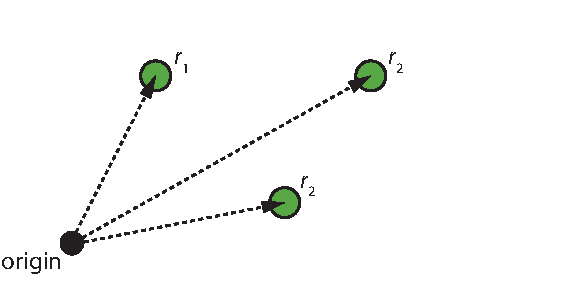
\includegraphics[width=\textwidth]{position_vectors_1}
    \caption[Network2]%
      {{\small Defining atomic positions requires knowing both distance and direction with respect to some reference \emph{origin}.}}    
    \label{fig:position_vectors_1}
  \end{subfigure}
  \hfill
  \begin{subfigure}[t]{0.475\textwidth}  
    \centering 
    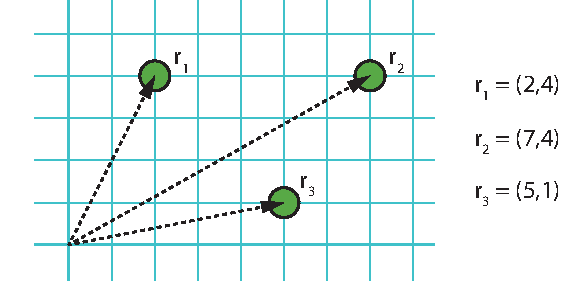
\includegraphics[width=\textwidth]{position_vectors_2}
  \caption[]%
      {{\small Describing positions using Cartesian coordinates, i.e.\ $(x,y)$ coordinates in two dimensions, or $(x,y,z)$ in three dimensions.}}    
    \label{fig:position_vectors_2}
  \end{subfigure}
  \vskip\baselineskip
  \begin{subfigure}[t]{0.475\textwidth}   
    \centering 
    \includegraphics[width=\textwidth]{position_vectors_3}
    \caption[]%
      {{\small The choice of coordinate system implicitly defines \emph{basis} vectors, $\vec{i}$ and $\vec{j}$. Any position can be expressed as a linear combination of these basis vectors.}}    
    \label{fig:position_vectors_3}
  \end{subfigure}
  \quad
  \begin{subfigure}[t]{0.475\textwidth}   
     \centering 
     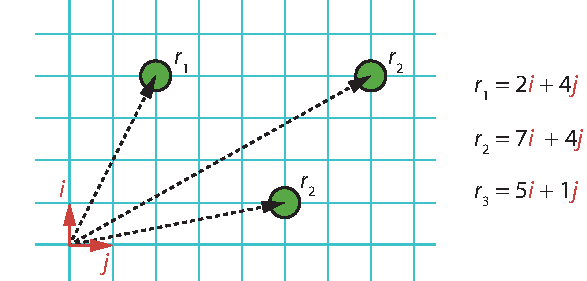
\includegraphics[width=\textwidth]{position_vectors_4}
     \caption[]%
       {{\small The $(x,y)$ coordinates given in \ref{fig:position_vectors_2} are the coefficients used to define each position in the basis $(\vec{i},\vec{j})$.}}    
     \label{fig:position_vectors_4}
   \end{subfigure}
 \caption
   {} 
 \label{fig:position_vectors}
\end{figure*}
A common choice for describing atomic positions is to use Cartesian coordinates, i.e.~$(x,y)$ in two dimensions, or $(x,y,z)$ in three dimensions \footnote{A good choice of coordinate system depends on the problem at hand, and Cartesian coordinated may not always be easiest to work with. For example, problems with spherical symmetry, such as describing atomic orbitals, will often be simpler when expressed in spherical coordinates $(r, \phi, \theta)$.}; this will be familiar from the interatomic distances (week 2) and molecular rotation (week 4) problems. In two dimensions, any position can be described by giving both the $x$ coordinate and the $y$ coordinate. Using the language of vectors, this choice of $x$ and $y$ coordinates defines a pair of \emph{basis} vectors, which we will denote $\vec{i}$ and $\vec{j}$. $\vec{i}$ is a vector of length $1$ pointing along $x$ and $\vec{j}$ is a vector of length $1$ pointing along $y$. Any position vector $\vec{r}=(x,y)$ can be expressed as a \emph{linear combination} of these basis vectors, i.e.\ $\vec{r} = x \times \vec{i} + y \times \vec{j}$. This means one way to think about the usual notation $(x,y)$ is that the two numbers describe the coefficients of $\vec{i}$ and $\vec{j}$ for a given linear combination. This might seem an overly complicated way of thinking about coordinates in Cartesian space, but it highlights that writing down a position vector such as $(3,4)$ is only meaningful if the basis vectors are defined. If we had chosen a different set of basis vectors, the \emph{same} positions would be described with \emph{different} vectors.
\begin{figure}[tb]
  \centering
  \resizebox{7cm}{!}{\includegraphics*{position_vectors_alternate_basis.pdf}} %
    \caption{\label{fig:position_vectors_alternate_basis}The three positions from Fig.~\ref{fig:position_vectors}, in a different basis.}
\end{figure}

\subsection{Vector addition, subtraction, scaling, and ``multiplication''}
Vectors can be added together by adding the coefficients of each basis vector (Fig.~\ref{fig:vector_addition}). For example, adding together the vectors $\vec{v}_1=(5,1)$ and $\vec{v}_2=(2,4)$ gives us a new vector $\vec{v}_3=(7,6)$. \begin{figure}[htb]
  \centering
  \resizebox{7cm}{!}{\includegraphics*{vector_addition.pdf}} %
    \caption{\label{fig:vector_addition}Vector addition,.}
\end{figure}
This rule is explained by writing $\vec{v}_1$ as $(5\vec{i}+1\vec{j})$ and $\vec{v}_2$ as $(2\vec{i}+4\vec{j})$. Adding $\vec{v1}$ and $\vec{v2}$ then gives $\left[(5\vec{i}+1\vec{j})+(2\vec{i}+4\vec{j})\right]$ and common terms can be collected together to give $\left[(5+2)\vec{i}+(1+4)\vec{j}\right]=(7\vec{i}+6\vec{j})$. Subtracting one vector from another follows the same rules, but with the coefficients of each basis vector subtracted; e.g. $\vec{v}_1-\vec{v}_2=(3,-3)$. 

Scaling a vector involved multiplying by a \emph{scalar} (hence the name). This changes the length of the vector, but not the direction, and involved multiplying each of the basis vector coefficients by the scalar value. i.e.~$\vec{v}_\mathrm{1}=(2,3)$. $\vec{v}_1\times2=(4,6)$. Again, we can understand this by expanding out the original vector in terms of the basis vectors, $\vec{i}$ and $\vec{j}$: $(2\vec{i}+3\vec{j})\times2=(4\vec{i}+6\vec{j})$.

\subsubsection{The dot-product and the cross-product}
We can also ``multiply'' two vectors together, although this is more complex. In fact there are \emph{two} standard ways to define ``multiplication'' of vectors.

The \emph{dot product} is also known as the ``scalar product''. This operation takes two vectors and returns a scalar quantity. The dot product of two vectors is denoted $\vec{a}\cdot\vec{b}$, and is defined as
\begin{equation}
\vec{a}\cdot\vec{b} = \sum_ia_ib_i = a_1b_1 + a_2b_2 + \ldots + a_nb_n.
\end{equation}
For example, if $\vec{a}=(2,1)$ and $\vec{b}=(3,2)$ then $\vec{a}\cdot\vec{b}$ is given by
\begin{eqnarray}
\vec{a}\cdot\vec{b} & = & (x_\mathrm{a} \times x_\mathrm{b})+ (y_\mathrm{a}\times y_\mathrm{b})\\
& = & (2\times3 + 1\times2) \\
& = & 8
\end{eqnarray}
An equivalent definition of the dot product is
\begin{equation}
\vec{a}\cdot\vec{b} = \norm{\vec{a}}\norm{\vec{b}}\cos\theta,
\end{equation}
where $\norm{\vec{a}}$ is the \emph{length} of vector $\vec{a}$, and $\theta$ is the angle between $\vec{a}$ and $\vec{b}$.

The \emph{cross-product} is also known as the ``vector product''. This operation takes two vectors and returns a vector quantity, with magnitude and direction. The cross product between vectors $\vec{a}$ and $\vec{b}$ is denoted $\vec{a}\times\vec{b}$ and is defined as a vector \emph{perpendicular} to the plane containing $\vec{a}$ and $\vec{b}$ with a length given by the parallelogram with $\vec{a}$ and $\vec{b}$ as sides (Fig.~\ref{fig:cross_product}). 
\begin{figure}[tb]
  \centering
  \resizebox{7cm}{!}{\includegraphics*{cross_product.pdf}} %
    \caption{\label{fig:cross_product}The cross product of $\vec{a}$ and $\vec{b}$ is proportional to the area $A$ of the parallelogram with sides $\vec{a}$ and $\vec{b}$.}
\end{figure}
This can be computed as
\begin{equation}
\vec{a}\times\vec{b} = \norm{\vec{a}}\norm{\vec{b}}\sin\theta\,\vec{n},
\end{equation}
where $\vec{n}$ is the \emph{unit vector} (a vector with length 1) perpendicular to the plane containing $\vec{a}$ and $\vec{b}$.

\section{Working with vectors in Python}
Working with vectors in Python is made simple by using \texttt{numpy} arrays.
\begin{lstlisting}
import numpy as np

# define two 2D vectors using numpy arrays
a = np.array([5,1])
b = np.array([2,4])
print(a)
print(b)

# vector addition
c = a + b
print(c)

# vector subtraction
c = a - b
\end{lstlisting}
Remember that multiplication of \texttt{numpy} arrays involved element-wise multiplication and returns a new array.
\begin{lstlisting}
# vector multiplication?
d = a * b
print(d)
\end{lstlisting}
This is \emph{not} the same as $\vec{a}\cdot\vec{b}$ or $\vec{a}\times\vec{b}$. Instead we can use the \texttt{numpy.dot()} and \texttt{numpy.cross()} functions:
\begin{lstlisting}
# dot product
dot = np.dot(a,b)
print(dot)

# cross product
cross = np.cross(a,b)
print(cross)
\end{lstlisting}

\vspace{\baselineskip}
\begin{center}
  \noindent\fbox{%
      \begin{minipage}{0.9\textwidth}%
          \vspace{0.15\baselineskip}
      \subsubsection*{Exercise}
          In week 2 you wrote some code to calculate interatomic distances (and angles) between pairs of atoms in example molecules, using the expression
          \begin{equation}
          r_{ij} = \sqrt{(x_i-x_j)^2+(y_i-y_j)^2+(z_i-z_j)^2}.
          \end{equation}
          Starting from your week 2 code, or from scratch, write a new version of this code that solves the problem using \texttt{numpy} arrays and \texttt{np.dot}.

          The \texttt{molecule1.txt} and \texttt{molecule2.txt} files can be downloaded from Moodle.
      \end{minipage}
  }
\end{center}


%\bibliographystyle{rsc}
%\bibliography{handout_5}

\end{document}
